\vspace{-0.1in}
\section{Introduction}
% \vspace{-0.1in}



% Numerous strategies have been proposed to address the efficiency challenges in Large Language Models (LLMs)~\citep{zhu2023survey,ding2023efficiency}. 
In the realm of Large Language Models (LLMs) compression, various techniques have been extensively explored, including weight quantization~\citep{dettmers2022llm}, network pruning~\citep{frantar2023sparsegpt}, and knowledge distillation~\citep{agarwal2023gkd}. 
Distinct from these approaches, the paradigm of low-rank matrix decomposition is less explored in LLMs but holds significant promise. Decomposition involves approximating the weight matrices in neural networks with matrices of lower rank, effectively reducing the model size. Given the massive number of parameters in LLMs, low-rank decomposition offers significant potential for memory reduction. 
Furthermore, low-rank decomposition can complement existing LLM compression techniques by further compressing quantized or pruned models, enhancing overall efficiency~\citep{cheng2017survey}.
% Despite its potential, it remains a relatively underutilized approach for LLM compression. 


From the perspective of network compression, traditional low-rank decomposition methods typically adhere to a straightforward process: initially training the original model and subsequently fine-tuning the decomposed model~\citep{jaderberg2014speeding,khodak2021initialization,wang2021pufferfish,hsu2022language}. While this approach is effective, it is resource-intensive and requires the entire training dataset and substantial computational power for end-to-end backpropagation. Applying this method to LLMs would encounter major challenges. Firstly, the training data for LLMs may not always be readily available, often restricted by privacy and commercial considerations. Secondly, the training process for these models is notoriously expensive, both in terms of time and computational resources. 

Given these constraints, the concept of ``training-free'' compression emerges as a more viable approach for LLMs~\citep{zhu2023survey}. This approach includes methods like LLM post-training quantization~\citep{dettmers2022llm,yuan2023rptq} and LLM post-training pruning \citep{frantar2023sparsegpt}, which compress LLMs without the need for extensive retraining.
These training-free (\textit{i.e., post-training}) methods offer a more practical solution for efficiently compressing LLMs. 

%while circumventing the limitations of traditional low-rank decomposition techniques.


To realize \textbf{LLM low-rank decomposition in a training-free manner}, we conduct an extensive analysis of the baseline methods for LLM decomposition. 
We first observe that straightforward application of existing low-rank decomposition techniques, which typically necessitate training, turns out ineffective for LLMs~\citep{denton2014exploiting,lebedev2014speeding,sainath2013low,moczulski2015acdc,jaderberg2014speeding,khodak2021initialization,wang2021pufferfish}. 


Digging into the failures, we reveal two challenges to post-training decomposition for LLMs. \raisebox{-1.1pt}{\ding[1.1]{182\relax}} Managing activation distribution in LLMs: This challenge involves addressing outliers in the activations, which can intensify the decomposition error. The importance of handling such outliers in LLMs echoes findings in recent quantization research \citep{lin2023awq,kim2023squeezellm}. These outliers can disproportionately affect the accuracy of matrix approximations, leading to suboptimal compression results.
\raisebox{-1.1pt}{\ding[1.1]{183\relax}} Balancing layer's decomposition sensitivity: Some layers are more sensitive to the decompostion than others, and decomposing them uniformly can lead to significant performance degradation. The key challenge is to balance the sensitivity of each layer with the efficiency of the whole network's decomposition.

\begin{figure}
\vspace{-0.2in}
\begin{minipage}{\textwidth}
    \begin{subfigure}{0.44\textwidth}
    \centering
    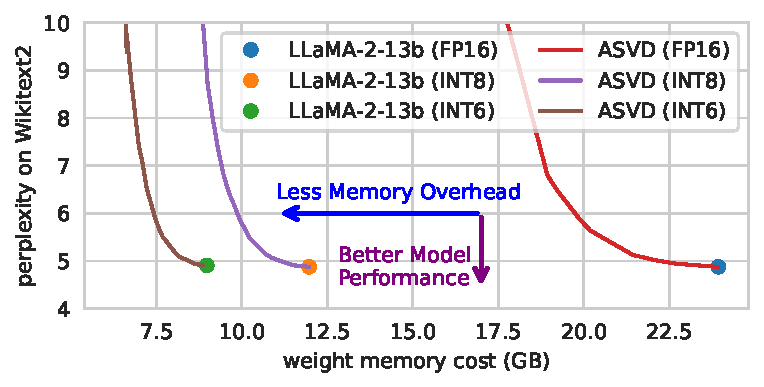
\includegraphics[width=\textwidth]{ims/intro-performance3.pdf}
    \caption{Summarized Performance of \asvd.}
    \label{fig:performance-summary}
    \end{subfigure}
    \hfill
    \begin{subfigure}{0.53\textwidth}
    \centering
    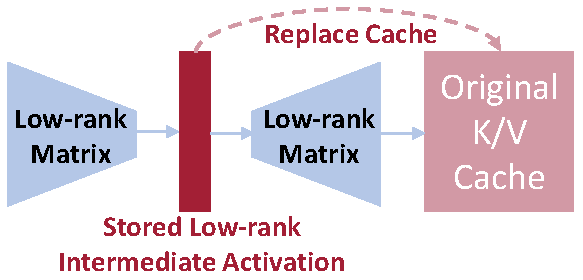
\includegraphics[width=0.9\textwidth]{ims/kvcompression-brief-crop.pdf}
    \caption{High-level idea of using \textit{\asvd~to compress KV cache}.}
    \label{fig:kvcompression-idea}
    \end{subfigure}
    \end{minipage}
    \vspace{-0.1in}
  \caption{\small \textbf{(a)} Our post-training LLM decomposition method is \textbf{orthogonal} to existing LLM compression techniques, enabling it to function as a versatile and plug-and-play solution for prevalent compression paradigms, including popular quantization methods. \textbf{(b)} By applying low-rank decomposition via \asvd~to the Key/Value projection matrices, the original high-dimensional \textbf{KV cache} can be replaced with a low-dimensional storage.}
  \vspace{-0.2in}
\label{fig:intro}
\end{figure}
Targeting challenge \raisebox{-1.1pt}{\ding[1.1]{182\relax}}, we propose the activation-aware decomposition method, where the distribution of activations are considered into the weight decomposition process. 
Specifically, we transform the values in the weight matrix column-wisely via a scaling matrix. The scaling matrix is designed based on the distribution patterns observed across input activation channels. This adjustment proves particularly beneficial for activation with outliers, allowing the decomposition to allocate enhanced focus to these specific weights. 
% Such targeted adjustment facilitates a more accurate reconstruction of the weight matrix, thereby minimizing prediction errors and improving the overall efficiency of the decomposition process.
Targeting challenge \raisebox{-1.1pt}{\ding[1.1]{183\relax}}, we further investigate the varying sensitivity of different LLM layers to decomposition. We find that weights in Multi-Head Attention layers ~\citep{vaswani2017attention} tend to be more resilient to decomposition compared to those in Multi-Layer Perceptron layers. This sensitivity variability across layers prompts us to develop a method to assign the compression ratio for each layer. 
\asvd~assesses each layer's sensitivity to decomposition at different ranks, enabling us to assign a suitable rank for optimal decomposition. Note that this probing assess is very efficient, requiring only a limited sample set for evaluation. 

Our experiments reveal that \asvd~can reduce the rank of the weight matrix by 10\% to 90\% in different layers, and it can achieve compression of model size 10\%-30\% in LLaMA models~\citep{touvron2023llama1,touvron2023llama2}.
We also validate \asvd~is compatible with 4/8-bit weight quantization, which is described in Sect.~\ref{sec:quantization}. 

Importantly, leveraging the successful low-rank decomposition of projection matrices in the self-attention module, we can integrate \asvd~with KV cache compression. 
Specifically, by applying \asvd~to decompose the Key/Value projection matrices, we can derive low-rank intermediate activations that serve as replacements for the KV cache stored in a high-dimension space, as shown in Fig.~\ref{fig:kvcompression-idea}. This substitution significantly reduces the memory usage of the KV cache, enabling support for larger batch sizes or longer sequence lengths, which are essential for real-world applications~\citep{yuan2024llmunveiled}.
In practice, by replacing the KV cache with intermediate low-rank activations, we can reduce up to 50\% of the memory consumption of the KV cache.

\vspace{-0.1in}